

For each form of environmental fluctuation and the stable non fluctuating environment, we performed 50 simulations, each on 500000 iterations with the parameters listed in Table~\ref{settings}. We report average value with standard deviations.

\begin{table}
\scriptsize
\centering
\begin{tabular}{l>{\centering}p{0.2\columnwidth}}\toprule%
Parameter & Value \tabularnewline
\toprule%
Number of living states & 5\tabularnewline
Successive living iterations before decay & 7\tabularnewline
Number of iterations for decay & 375-1875\tabularnewline
Direct transition to decay & enabled\tabularnewline
Size of the grid & 500x500\tabularnewline
Grid boundaries & toric grid\tabularnewline
Transition Rule~(TR) & CA-LGP\tabularnewline
Maximum (TR) size & 50 program statements\tabularnewline
Genotype copy neighbouring  & Von Neumann \tabularnewline
Transition rule neighbouring & Moore\tabularnewline
\bottomrule%
\end{tabular}
\caption{ \textbf{HetCA parameters}.}
  \label{settings}
\end{table}

\subsection{Genotype Size}
We use the number of program statements ($n_{prog}$) as a measure of the genotype size and compute the average size of all the current genotypes of a run every 2500 iterations. We then report the average and standard error among all the fifty runs sharing the same settings.

\subsection{Changes induced by environmental fluctuation}
If, as postulated in \citep{jablonka2014evolution}, the introduction of environmental changes leads to the selection of plasticity or to the emergence of phenotypic selections\footnote{Similar to the epigenetic inheritance system} using easily reversible phenotypic mutations, then phenotypes from different individuals of the same lineage observed while environmental conditions are similar should be relatively close even though individuals from their lineage evolved in other environmental conditions between these measures. While, if the adaptation to each environmental change is done exclusively through the selection of classical irreversible genotypic mutations, these phenotypes shall be quite different, despite the potential evolutionary convergence. That is why we want to develop a metric to measure phenotypic proximity between two iterations of the CA. To do this we simply compare the proportions of living cells in different states among the possible states. The phenotypic difference $\sigma(t_1,t_2)$ between two iterations $t_1$ and $t_2$ is then calculated as:
$$\sigma(t_1,t_2) = \sum_{s=1}^5 | \frac{N(s,t_1)}{\sum_{s=1}^5 N(s,t_1)}-\frac{N(s,t_2)}{\sum_{s=1}^5 N(s,t_2)}|$$ where $N(s,t)$ is the number of cells at the state $s$ for iteration $t$.

Every 5000 iterations $t$ of the CA we perform two phenotypic comparison with an iteration $t'$ such as $t'\in[t-55000;t-60000]$. The first phenotypic comparison aims to compare two similar environment and therefore we choose $t'$ such as $E(t')=E(t)$. The second phenotypic comparison aims to compare two disimilar environment and therefore we choose $t'$ such as $E(t')=E(t+f)$.  

\subsection{Density}
We also collect the \emph{most common genotype}~(most frequently occurring) in iterations 2500\footnote{\citep{medernach2015evolutionary}  has shown that the most common genotypes during the first iterations of HetCA were unlikely to have a viable survival strategy, therefore we chose to collect genotypes from iteration 2500.}, 102500, 202500, 302500, 402500 and 500000. 

\subsection{Regular phenotype characterization} 
In HetCA, to survive in the long term the genotypes must regularly release cells by transforming them into quiescent cells without genotypes. This generates patterns and cycles which are quite easy to observe in homogeneous simulations where a single genotype is tested as shown in Figure~\ref{foursteps}, but also observable, although with more difficulty, in normal, heterogeneous, HetCA simulations as seen in Figure~\ref{fourstepsreal}. That is why, characterize phenotypes, we found it useful to measure these cycles as well as out-of regularities. At every iteration $t>8$ of the homogenous genotype test, we compare the states $S_t$ and $S_{t-1}$ of each cell to their anterior state during the eight previous iterations of the CA. We then measure whether this sequence of two states is repeated during these eight previous iterations, and if so what is its periodicity $p$ such as $p=\min p \in [2;7], S_t=S_{t-p} \wedge S_{t-1}=S_{t-1-p}$. We use here a sequence of two states because, if the genotype of a cell adopts a stable strategy, i.e. repeats a sequence of states, this sequence must contain a minimum of two states in order to ensure the survival of the genotype -- the quiescent state and one of the living states. We have chosen to limit ourselves to a comparison of the eight previous iterations as the limit of the seven consecutive live iterations before decay involves a maximum periodicity of quiescent state of seven iterations. We have chosen to limit ourselves to a comparison of the eight previous iterations to reduce the computational cost and because the limit of the seven consecutive live iterations before decay involves, for a successful regular phenotype, a maximum periodicity of seven iterations for the quiescent state. We perform this measure only if there is at least a living state among the last two states and no state decay. We then report, for each iteration $t$ of the CA, the sum $\Sigma(p,t)\forall p \in [2;7]$ of cells at every possible periodicity $p$. 

\subsection{Phenotype disturbance} 
To analyze the phenotypic plasticity and / or the existence of phenotypic selection it is necessary to have a measure of the stability of the phenotype. To achieve this, in each iteration $t$ we compare the periodicity $p_t$ of each cell to its previous periodicity $p_{t-1}$. We then report, for each iteration $t$ of the CA, the number of cells that changed periodicity.
 
\begin{figure}[h]
\centering
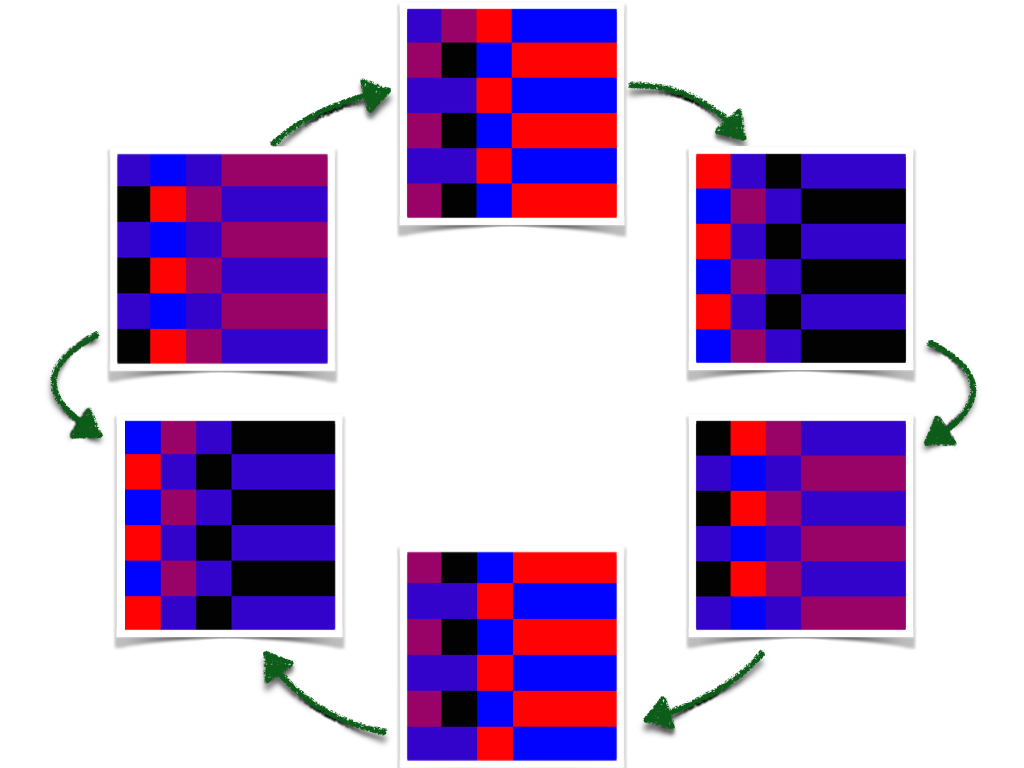
\includegraphics[width=0.5\columnwidth]{img/4steptransition}
\caption{\textbf{Six steps survival strategy} from a genotype extracted from a HetCA simulation in a stable environment and tested here in a randomly initialized homogenous CA. }
  \label{foursteps}
\end{figure}
 
\begin{figure}[h]
\centering
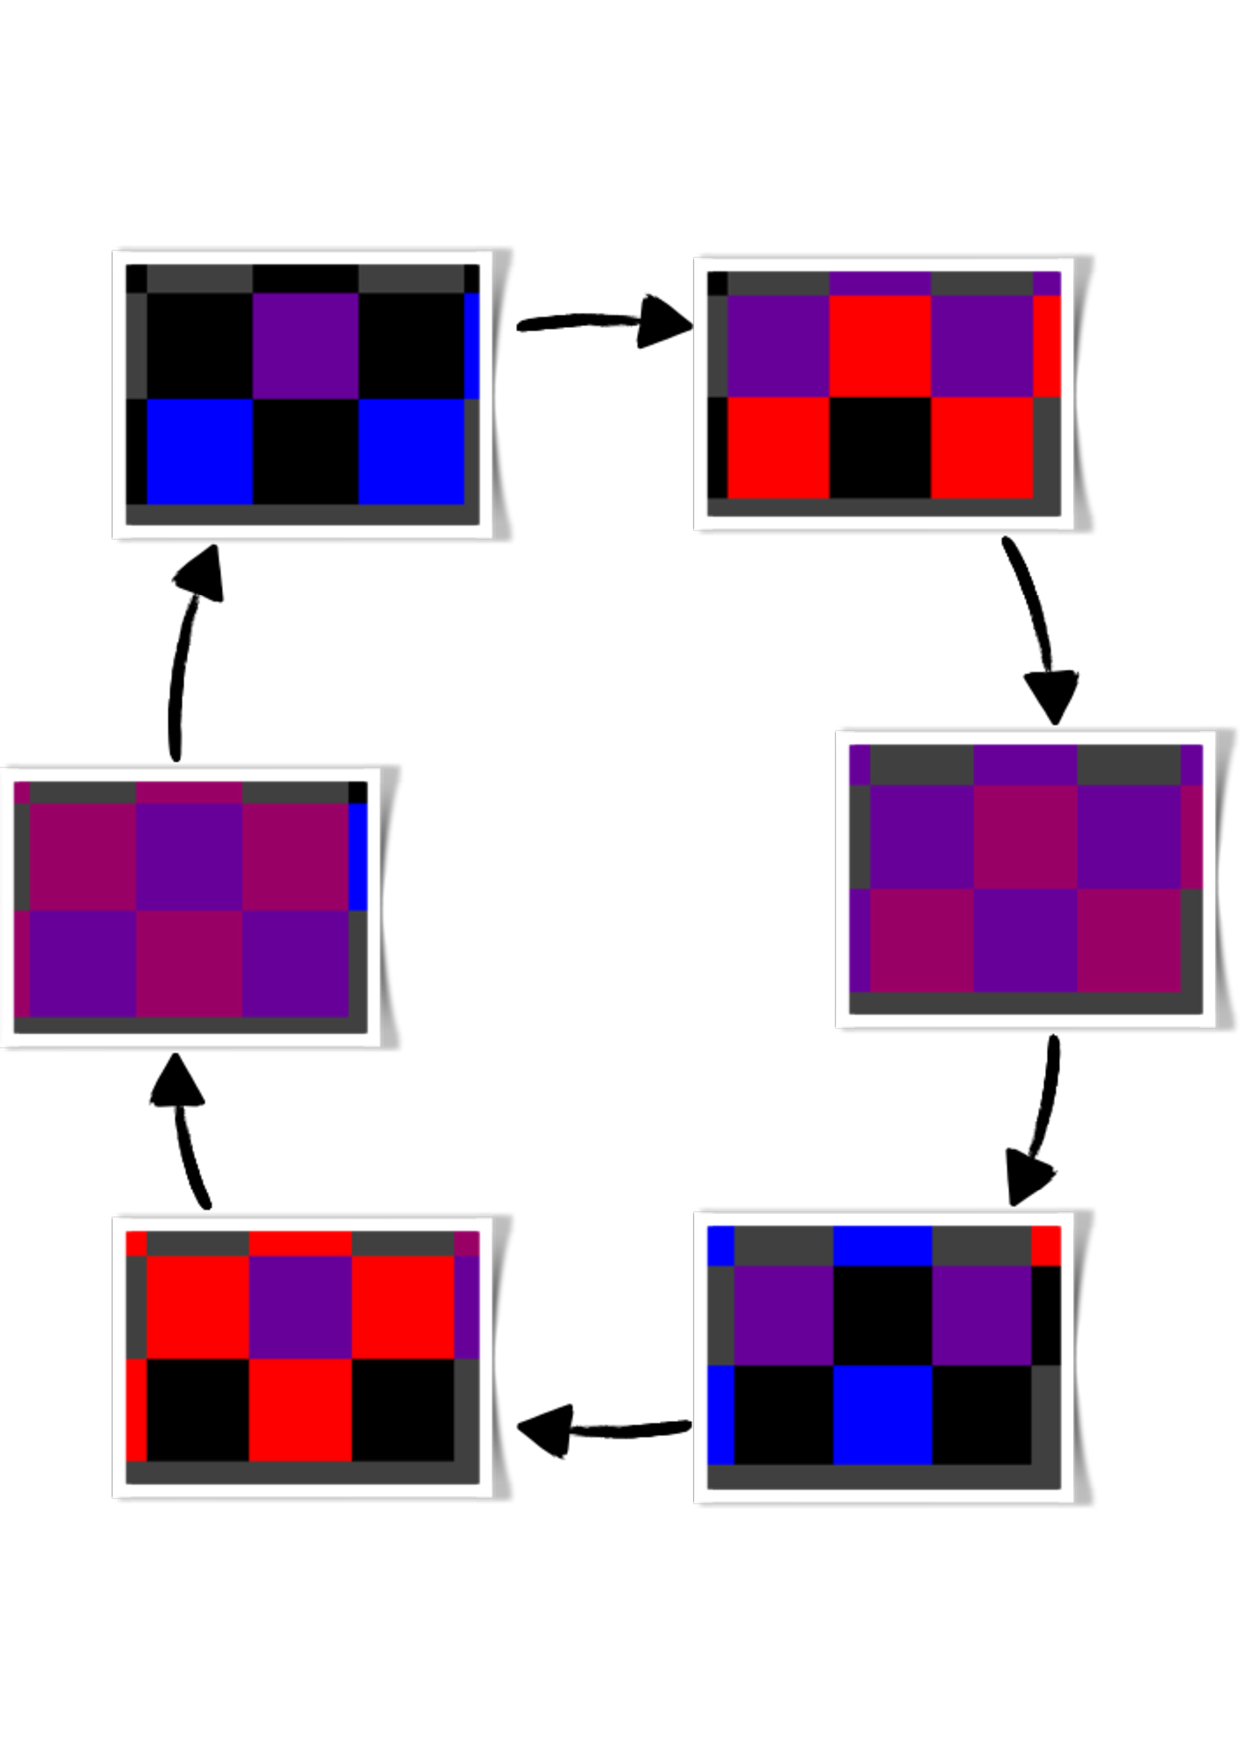
\includegraphics[width=0.5\columnwidth, angle =-90]{img/cyclesReal}
\caption{\textbf{Six steps survival strategy} from a HetCA simulation with \emph{Short-cycle Fluctuation}. }
  \label{fourstepsreal}
\end{figure}






